\chapter{HIL felépítése}

Nyilvánvaló tehát, hogy napjainkban, a modern teljesítmény elektronikai eszközök fejlesztéséhez elengedhetetlen a HIL szimulátor alkalmazása. Bár az eszköz fejlesztése jelentős terhet ró a készítőkre, segítségével csökkenthető a tervezésre fordítandó idő, a fejlesztési folyamatok párhuzamosításával. Segítségével elkerülhetőek a költséges és veszélyes hibák a fejlesztés alatt, hiszen a teljesítmény elektronikai elemek csak matematikai modell formájában jelennek meg a rendszerben. Ezen felül a tesztelés minősége is jelentősen javítható a költségek csökkentése mellett. Ilyen szimulátorból sok futhat egymás mellett párhuzamosan, a valós elektronika többszöri felépítése nélkül. Így sok különböző teszteset futtatható egyszerre, akár ciklikusan, emberi felügyelet nélkül. \cite{sutozoli}\cite{low_cost_rt_hil}\cite{hw_emu}

\section{Hardware felépítése}

A HIL szimulátor hardver nem más, mint egy interfész elektronika a vezérlő hardverek és a szimulációt végző FPGA között. \Afigref{hw_architect} ábrán láthatóak a vezérlést végző elemek. A HIL szimulátor feladata a bal oldali, Power Subsystem blokkból érkező jelek előállítása, illetve a vezérlő jelek fogadása.

/todo[inline]{Lehetne részletezni talán}

\subsection{CCB és MCB csatlakozó}
\todo[inline]{Meg kell rendesen foglalmani a kis mondandóm}
A szimuláció során a PIB nem szükséges, ezért az MCB és a CCB kapcsolatát is a HIL elektronika biztosítja. A két eszköz között a kommunikáció UART vonalon valósul meg. A kivitelezés számomra több szempontból is érdekes, mert a sebesség $9\ Mbaud$, illetve a fizikai réteg sem teljesen szokványos. Az UART jelek differenciálisan kerülnek átvitelre az MCB felé, de az Rx és a Tx egy-egy külön érpárt kapott. Az MCB-n keresztül érkeznek még ezen felül a \emph{Sto1X} és a \emph{Sto2X} jelek. Ezek a jelek szintén speciálisak, az eszköz vészleállításáért felnek. A CCB-vel való kommunikáció \aref{table:ccbsignals}. táblázatban felsorolt jelek segítségével valósul meg. 

\begin{table}[]
\centering
\begin{tabular}{|l|l|l|l|}
\hline
\textbf{Név}   & \textbf{I/O} & \textbf{A/D} & \textbf{Leírás}                 \\ \hline
UoutU          & Digital      & Bemenet      & Az U fázis nullátmenetének jele \\ \hline
UoutV          & Digital      & Bemenet      & A V fázis nullátmenetének jele  \\ \hline
UoutW          & Digital      & Bemenet      & A W fázis nullátmenetének jele  \\ \hline
Sto1SatusX     & Digital      & Bemenet      &                                 \\ \hline
Sto2SatusX     & Digital      & Bemenet      &                                 \\ \hline
MCB\_TxD       & Digital      & Kimenet      &                                 \\ \hline
MCB\_RxD       & Digital      & Bemenet      &                                 \\ \hline
EEPROM\_SDA    & Digital      & Be/Kimenet   &                                 \\ \hline
EEPAROM\_SCL   & Digital      & Kimenet      &                                 \\ \hline
RectStatusC    & Digital      & Bemenet      &                                 \\ \hline
PrechargeCtrlX & Digital      &              &                                 \\ \hline
IgbtBFltX      & Digital      &              &                                 \\ \hline
IgbtBRdy       & Digital      &              &                                 \\ \hline
IgbtBRstX      & Digital      &              &                                 \\ \hline
IgbtPsuCtrlX   & Digital      &              &                                 \\ \hline
IgbtInvFltX    & Digital      &              &                                 \\ \hline
IgbtInvRdy     & Digital      &              &                                 \\ \hline
IgbtInvRstX    & Digital      & Kimenet      &                                 \\ \hline
IgbtU1         & Digital      & Kimenet      &                                 \\ \hline
IgbtU2         & Digital      & Kimenet      &                                 \\ \hline
IgbtV1         & Digital      & Kimenet      &                                 \\ \hline
IgbtV2         & Digital      & Kimenet      &                                 \\ \hline
IgbtW1         & Digital      & Kimenet      &                                 \\ \hline
IgbtW2         & Digital      & Kimenet      &                                 \\ \hline
IgbtB          & Digital      & Kimenet      &                                 \\ \hline
FanPsuCtrC     & Digital      & Kimenet      &                                 \\ \hline
FanExtCtrC     & Digital      & Kimenet      &                                 \\ \hline
FanIntCtrC     & Digital      & Kimenet      &                                 \\ \hline
FanExtSpeedC1  & Digital      & Kimenet      &                                 \\ \hline
FanExtSpeedC2  & Digital      & Kimenet      &                                 \\ \hline
TIgbtW         & Analog       & Bemenet      &                                 \\ \hline
15VCM          & Analog       & Bemenet      &                                 \\ \hline
TIgbtV         & Analog       & Bemenet      &                                 \\ \hline
UdcMN          & Analog       & Bemenet      &                                 \\ \hline
UdcMP          & Analog       & Bemenet      &                                 \\ \hline
IWN            & Analog       & Bemenet      &                                 \\ \hline
IWP            & Analog       & Bemenet      &                                 \\ \hline
TIgbtU         & Analog       & Bemenet      &                                 \\ \hline
TIgbtB         & Analog       & Bemenet      &                                 \\ \hline
IUP            & Analog       & Bemenet      &                                 \\ \hline
IUN            & Analog       & Bemenet      &                                 \\ \hline
IVP            & Analog       & Bemenet      &                                 \\ \hline
IVN            & Analog       & Bemenet      &                                 \\ \hline
TA             & Analog       & Bemenet      &                                 \\ \hline
5VSto1         & Analog       & Bemenet      &                                 \\ \hline
5VSto2         & Analog       & Bemenet      &                                 \\ \hline
UdcP           & Analog       & Bemenet      &                                 \\ \hline
UdcN           & Analog       & Bemenet      &                                 \\ \hline
\end{tabular}
\caption{A CCB jelei}
\label{tab:ccbsignals}
\end{table}

Ezek azok a jelek, amiket a HIL-nek vagy szimulálnia, vagy pedig fogadnia kell. Ezen felül található a csatlakozón még két \emph{5V\_Loopback} nevű láb, ezt a táblázatban nem szerepeltettem. Ennek az a funkciója, hogy létre lehet hozni a PIB-en olyan áramköri részeket, melyek az $5\ V$-os táplálást csak a CCB-n keresztül kapják meg, így nem indulnak el csatlakoztatott kártya nélkül.

A digitális jelek átvitele esetében a feladat egyszerű, csak a CCB és az FPGA közti jelszint különbséget kell megoldani. Ebben egy \emph{74LVC8T245PW} típusú level-shifter lesz segítségünkre. A CCB a jeleket $5\ V$-os tartományban adja ki, illetve fogadja, az FPGA maximális kimeneti feszültsége $3,3\ V$, és nem is állnak rendelkezésre nagyobb feszültséget toleráló lábak. A kisebb feszültségre való átalakításra lehetséges megoldás a feszültség osztó is, de a nagy sebességű jelek dinamikájának megőrzése érdekében inkább itt is a level-shiftert választottam. A lassabb jelek esetében maradtam a feszültség osztóval való megoldásnál.

Analóg jeleket tekintve csak bemenet található a CCB-n. Ezen jelek előállítását Sigma-Delta átalakítók segítségével oldottam meg, melyről részletesebben később lesz szó.

A fent említett jeleken kívül a HIL-en elhelyezésre került az ULINK és az St-Link debuggerek csatlakozója is, a fejlesztés kényelmesebbé tételének érdekében. A CCB-re a JTAG jelei egy külön flat-flex kábel segítségével csatlakoznak. Ennek a mechanikai teherbírása igen alacsony, így pedig nem kell egy külön kártyára csatlakoztatni, kockáztatva ezzel az elmozdulást, kontakthibát vagy vezeték szakadást.

\begin{figure}[!ht]
	\centering
	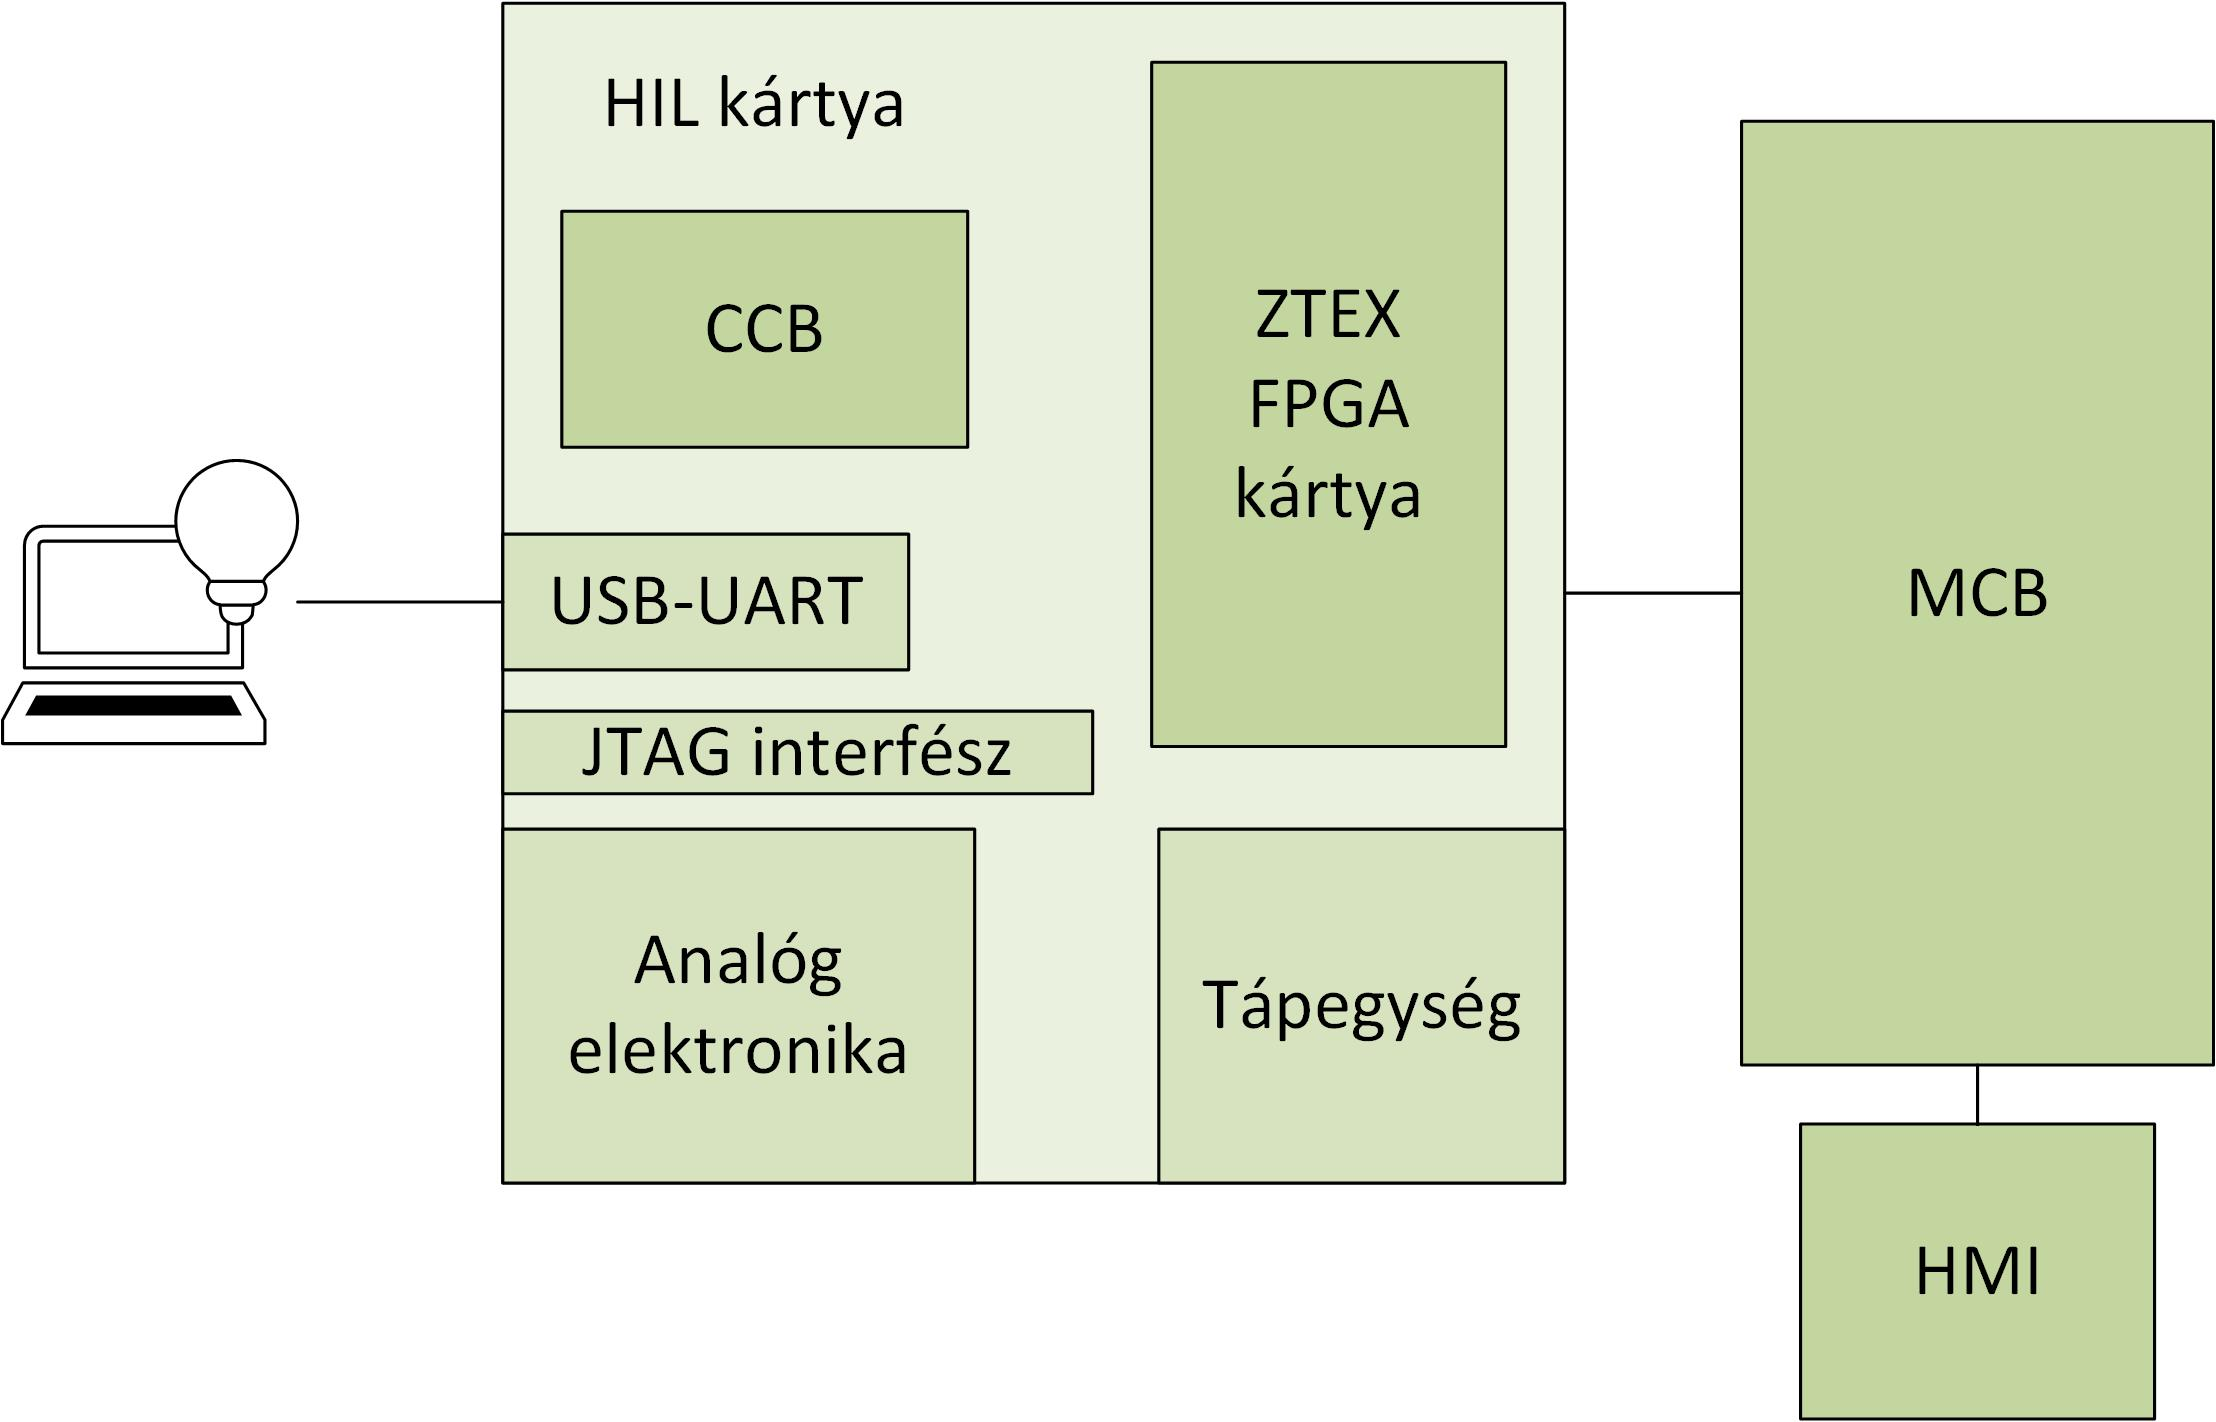
\includegraphics[width = 0.8\textwidth]{figures/hil.jpg}
	\caption{A HIL vázlatos felépítése} 
	\label{fig:hil_block}
\end{figure}

\subsection{Tápegység}
A kártya $24 V$-os tápfeszültségre lett tervezve. Ebből egy Linear Technologies \emph{LT3845AEFE#PBF} típusú szinkron buck tápegység vezérlő IC és a hozzá tartozó külső apparátus állítja elő az $5 V$-os táp feszültséget mind az FPGA mind pedig a CCB számára. A táp egység maximálisan $6 A$ terhelhetőségű, amely soknak tűnhet, de az FPGA fogyasztását jelentősen befolyásolja a benne található szoftver bonyolultsága, így elképzelhető a kapacitás teljes felhasználása is, kis teljesítmény esetén pedig hatékony tud maradni az úgynevezett \emph{Burst mode} működési mód segítségével.

\subsection{ZTEX kártya}

Egy ilyen teszt és fejlesztési eszköz készítése során az egyik legfontosabb szempont a modularitás. Nem láthatjuk előre feltétlenül, hogy a későbbiekben mire lesz szükség. Az FPGA önmagában biztosít modularitást, hiszen cserélhető benne a hardver, jelen esetben a megvalósított matematikai modell. Ezen felül egy közel 500 lábbal rendelkező BGA tokos FPGA-hoz a nyák tervezés sem triviális feladat. A megfelelő lábak kivezetéséhez legalább 6-8 rétegre van szükség, és nagyon sok hibalehetőséget tartogat magában. Ezek miatt egy FPGA modul alkalmazása mellett döntöttünk. Bár az elérhető GPIO lábak mennyisége így korlátozott, az FPGA-t működtető áramkör garantáltan üzemképes, illetve a saját tervezésű elektronika bonyolultsága is jelentősen csökken.

\begin{figure}[!ht]
	\centering
	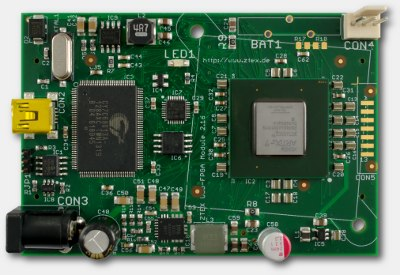
\includegraphics[width = 0.75\textwidth]{figures/fpga216.jpg}
	\caption{A ZTEX 2.16 FPGA board} 
	\label{fig:ztex}
\end{figure}

\Aref{fig:ztex} ábrán látható ZTEX panel mellett tettem le a voksom. A kártyáról kivezetésre kerültek a JTAG interfész jelei is, azonban az ehhez az FPGA-hoz való Xilinx debugger nem áll rendelkezésre. A ZTEX kártyán azonban egy Cypress mikrovezérlő segítségével, \emph{libusb} driver segítségével betölthető a bitstream mind a RAM-ba, ideiglenes teszthez, mind pedig a FLASH-be, melyből az FPGA minden indítás során be tudja olvasni azt.
/todo[inline]{Itt is lehet még részletezni a betöltés folyamatát}

\begin{figure}[!ht]
	\centering
	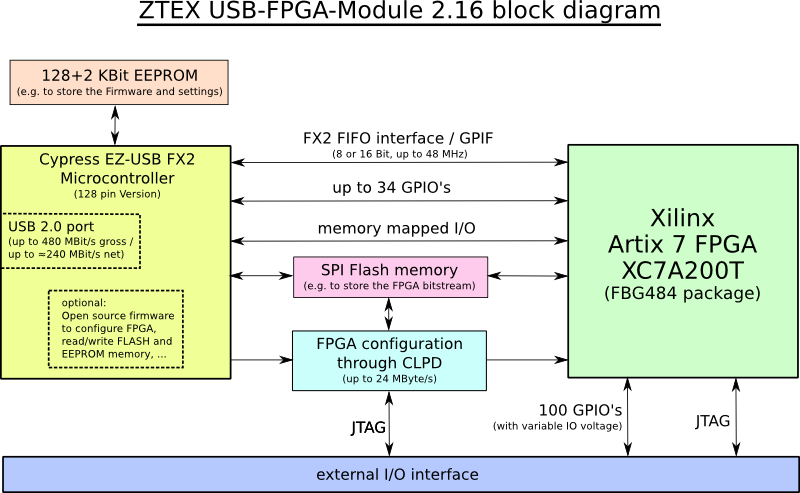
\includegraphics[width = 0.8\textwidth]{figures/usb-fpga-216.png}
	\caption{A ZTEX 2.16 FPGA board felépítése} 
	\label{fig:ztex_block}
\end{figure}

Ezen felül a rajta található Xilinx Artix 7 FPGA megfelelő hűtését is biztosítja a panel. Az FPGA főbb adatai \aref{table:artix7spec} táblázatban láthatóak. Ez az eszköz a Xilinx jelenleg kereskedelmei forgalomban kapható egyik zászlós hajója, amit bizonyít is a ZTEX panel 500 Eurós vételára.

\begin{table}[]
\centering
\begin{tabular}{ll}
Logikai cellák               & 215360 \\
Szeletek                     & 33650  \\
CLB Flip-flopok              & 269200 \\
Eloszott memória (kb)        & 2888   \\
Blokk RAM/FIFO (36 kb/darab) & 365    \\
Blokk RAM összesen (kb)      & 13140  \\
                             &        \\
                             &        \\
                             & 
  
\end{tabular}
\caption{A Xilinx Artix 7 XC7A200T}
\label{artix7spec}    
\end{table}

Bár a jelenlegi modell mindössze 10\%-át foglalja le a teljes hardvernek, a későbbi bővülésre is hagy lehetőséget. A frimware elkészítésére és fejlesztésére a Xilinx Vivado környezet biztosít lehetőséget. Ebben készült el a keret rendszer, mely a Simulink-ból generált HDL fájlokat tudja fogadni, megfelelő interfészen keresztül a kártyára vezetni.


\subsection{Szigma-Delta ($\Sigma{}\Delta{}$) átalakítók}

Az FPGA nem rendelkezik analóg kimentekkel, azonban a CCB számára elő kell állítani a normál működés során visszamért analóg jeleket, hiszen ebben rejlik a szimulátor lényege, a vezérlő elektronika szemszögéből nincsen különbség a valós hardver és a szimulátor között. A szigma delta átalakító nagyon nagy vonalakban egy órajel és egy fix impulzus szélességű négyszög jel, mely vagy logikai egy értéket, vagy logikai nulla értéket vesz fel az órajel minden felfutó (vagy lefutó) élére. Az így kialakult impulzus-sor kitöltési tényezője egy hosszabb mintavételi ablakot tekintve arányos a bemeneti kódszóval. Ezek után a jelet egy az órajelnél sokkal kisebb vágási frekvenciájú alul áteresztő szűrűvel feldolgozva analóg jelet kapunk. A szigma delta átalakító egyik előnye a PWM kimenethez képest, hogy a kvantálási zajt nagyfrekvenciás tartományba tolja. \cite{artofelectronics}

\todo[inline]{PWM vs sigma delta spektrum}

Igen félrevezető névvel szokás "1 bites DA" átalakítónak is nevezni. A kifejezés egyszerűséget és alacsony teljesítményt sugall, ennek ellenére a megoldás rendkívül lineáris és nagy felbontású eredményt ad, így elterjedten használják pl. audio eszközökben is.

A mi esetünkben két részre bontható az átalakító. A modellben fut egy analóg jelből digitális jelet létrehozó szigma-delta átalakító, majd az így kiadott digitális jelet szűrjük már az FPGA-n kívül egy alul áteresztő szűrűvel. \Aref{fig:sigmadelta} ábra szemlélteti az átalakító működését. A bejövő analóg jelből levonjuk a hiba jelet, majd egy komparátor összehasonlítja egy referenciával. Amennyiben nagyobb a bejövő jel, a kimenet logikai "1" értéket vesz fel, ha kisebb, logikai "0"-t. Ezt a jelet, egy 1-bites DAC-on keresztül vezetve akkumuláljuk, így kialakítva a hiba jelet. 

\begin{figure}[!h]
	\centering
	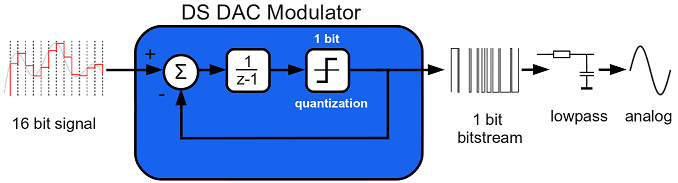
\includegraphics[width = 0.75\textwidth]{figures/first_oder_sd.png}
	\caption{A szigma-delta átalakító} 
	\label{fig:sigmadelta}
\end{figure}


\Aref{fig:nosie}. ábrán megfigyelhető, hogy hogyan változtatjuk meg a zaj spektrumát a szigma-delta átalakítás során. A $k$-szeres túlmintavételezés a zaj spektrumát elteríti a Nyquist frekvencia $k$-szeres tartományában, amivel már jelentős SNR növekedés érhető el. Ezután azonban a zajformázás még magasabb frekvencia tartományba tolja a zajt, melynek ezáltal az effektív értéke is növekszik, de ez nem probléma, mert a jel úgy is át fog haladni egy alul áteresztő szűrőn.

\begin{figure}[!h]
	\centering
	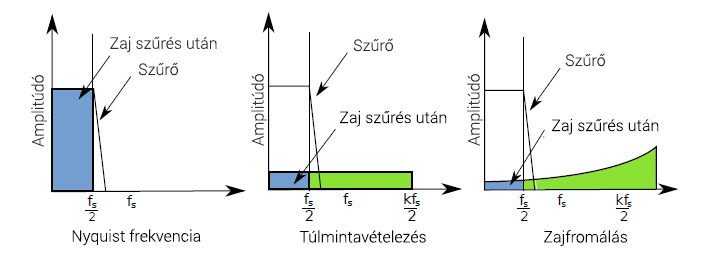
\includegraphics[width = \textwidth]{figures/noiseshape.png}
	\caption{A szigma-delta átalakító} 
	\label{fig:asd}
\end{figure}

Az így kapott jelet már a modellből az FPGA lábára vezethetjük. Mivel az FPGA kimeneti bankjainak feszültsége maximum $3,3\ V$, ezért a szűrés után erősítésre is szükség lehet.

\begin{figure}[!h]
	\centering
	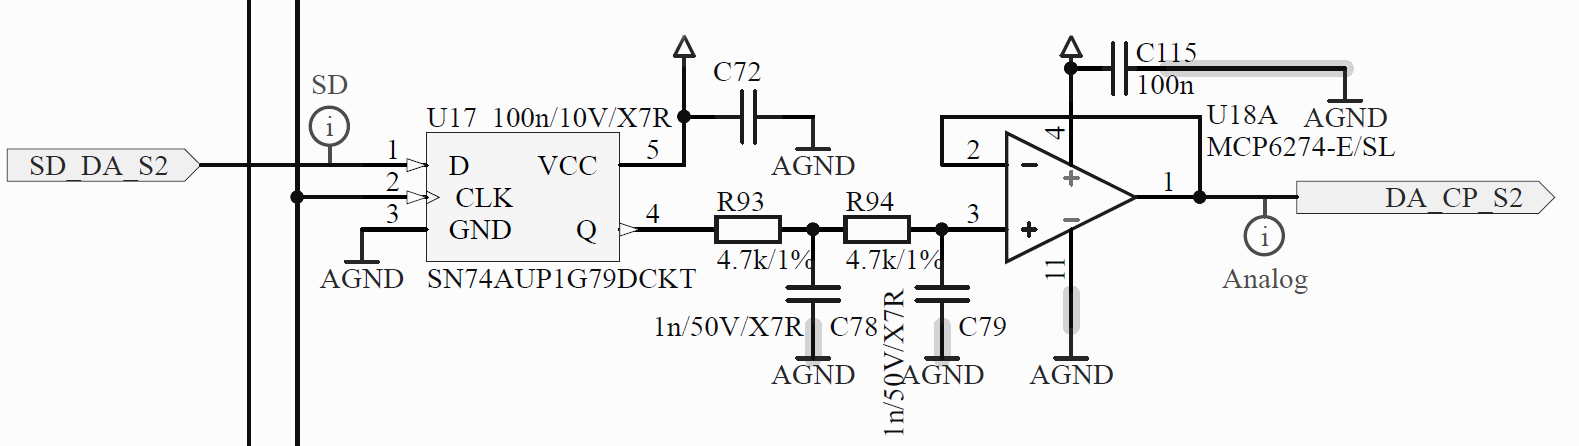
\includegraphics[width = \textwidth]{figures/lowpassfilter.png}
	\caption{A négyszögjelet fogadó aluláteresztő szűrő} 
	\label{fig:lowpass}
\end{figure}

\Aref{fig:lowpass} ábrán látható alul áteresztő szűrő kimenet már közvetlenül a CCB analóg bemenetére csatlakozik. A CCB analóg mérései differenciálisak a valóságban, mivel a valós elektronikában sokkal nagyobb zaj éri a rendszert. A modellen azonban ez a zavar nem jelentős, így a mérés negatív jelét földre kötöttem.

\begin{figure}[!h]
	\centering
	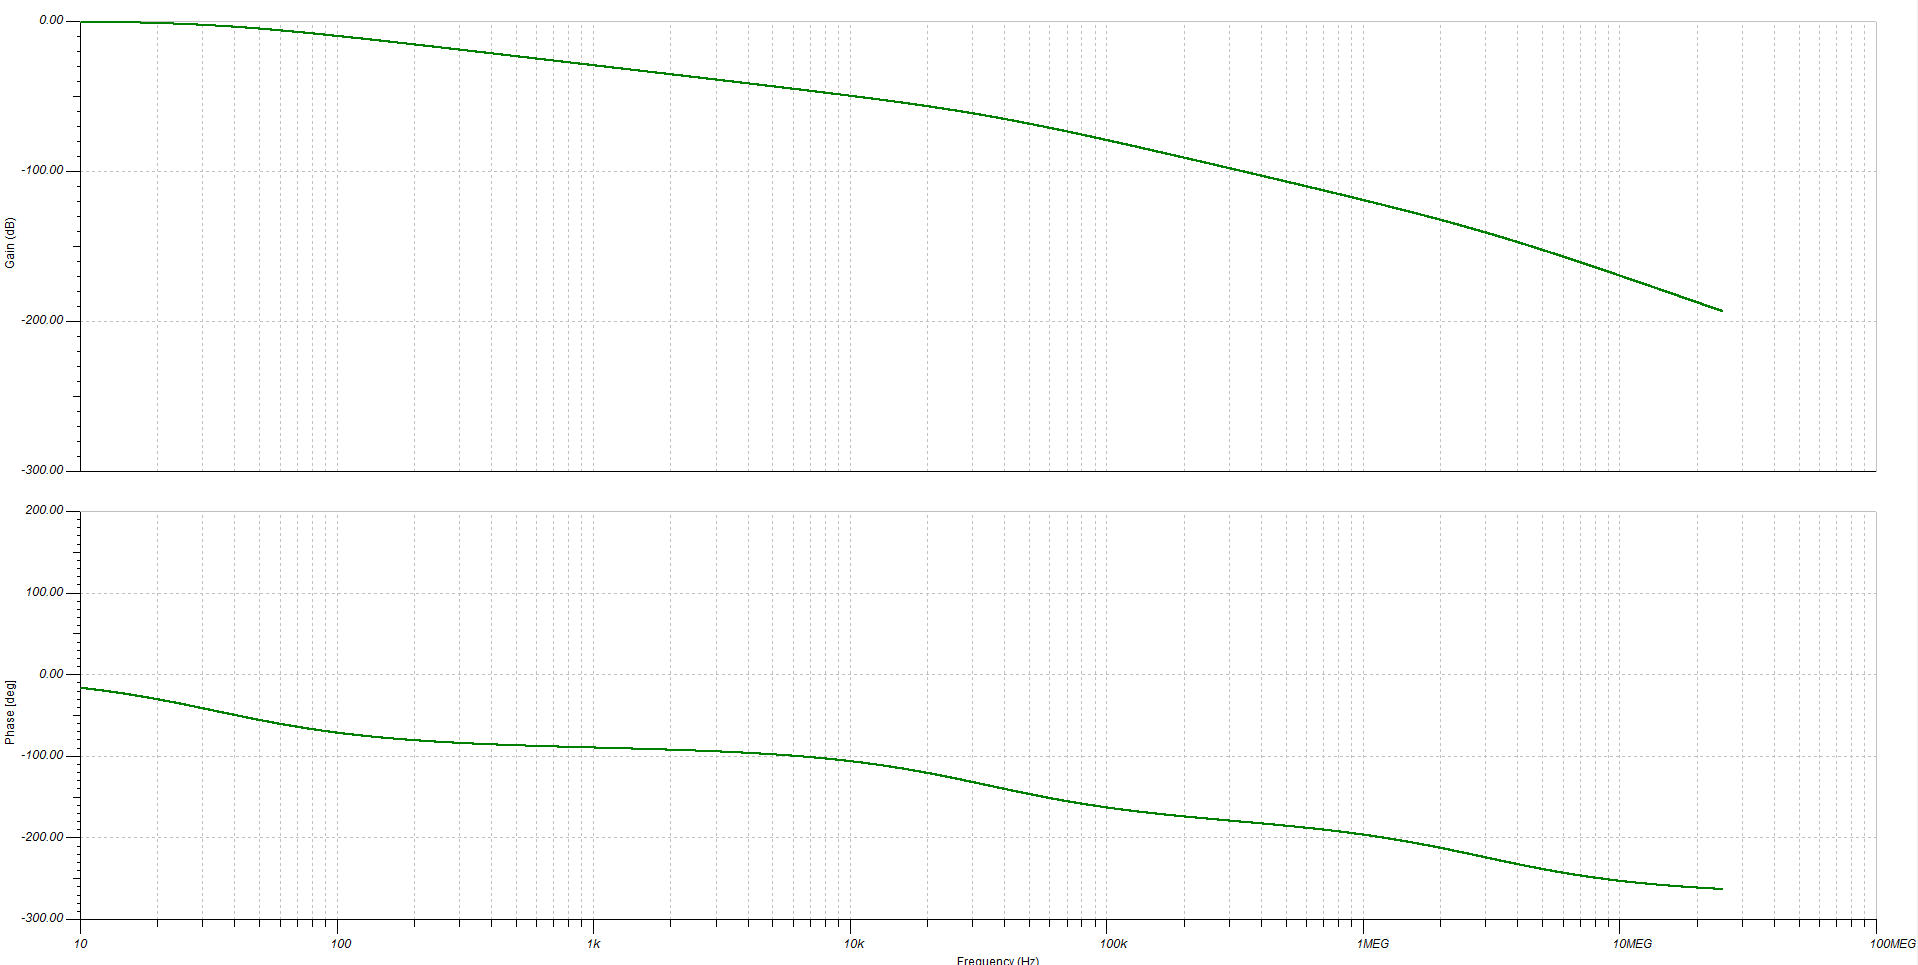
\includegraphics[width = \textwidth]{figures/sigma_delta_sim.png}
	\caption{Az aluláteresztő szűrő szimulációja TI Tina szoftver segítségével} 
	\label{fig:lowpass_sim}
\end{figure}

\Aref{fig:lowpass_sim}. ábrán látható a szűrő átvitelének szimulációja. Két töréspont látható a Bode-diagrammon $10\ Hz$ és $10\ kHz$ frekvenciánál. A szűrő méretezésénél figyelembe kell venni a kimeneti jelek sávszélességét, ami a mi esetünkben $1\ kHz$ alatt van, illetve a kimeneti négyszög jel frekvenciáját. Ez $18\ MHz$, így biztosak lehetünk benne, hogy a kimeneti jel az alkalmazás igényeinek megfelelő.

\subsection{Kiegészítő csatlakozó}

A könnyű bővítési lehetőségeket biztosítandó, a kártyán elhelyezésre került egy kiegészítő csatlakozó. Ennek segítségével később könnyedén kielégíthetőek lesznek most még nem látható igények. Az lábakon elérhető mind a $24\ V$-os, mind az $5\ V$-os táp feszültség, illetve a fel nem használt FPGA I/O-k vannak kivezetve. A lábak között kettőt dedikáltan I2C vonalnak használtam fel, itt a különbség mindössze annyi a többi lábhoz képest, hogy opcionálisan beforrasztható egy felhúzó ellenállás, illetve szintén forrasztható be soros impedancia. A csatlakozó pontos láb kiosztása \aref{fig:hil_extender}. ábrán látható.

\begin{figure}[!h]
	\centering
	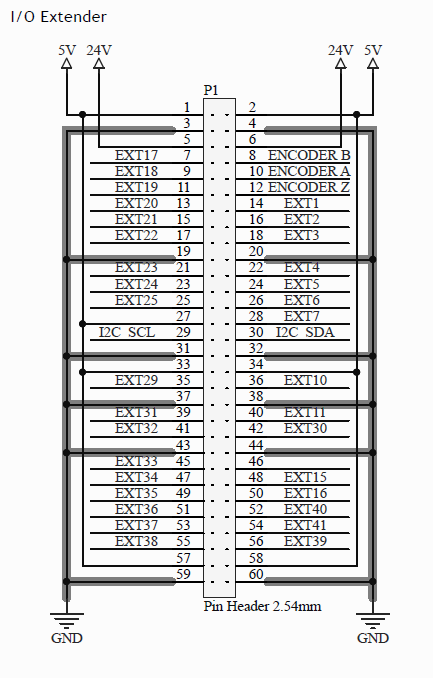
\includegraphics[width = \textwidth]{figures/hil_extender.png}
	\caption{A HIL kártya kiegészítő csatlakozója} 
	\label{fig:hil_extender}
\end{figure}

A kártya teljes kapcsolási rajza a dolgozat függelékében megtalálható.

\section{Simulink modell}

A futtatandó modell magában foglalja a teljesítmény elektronikai elemek modelljét, egy motor modellt és egy mechanikai terhelés modellt. Hiányossága volt azonban, hogy a DC-link feszültsége egy konstans érték volt, így a különböző terhelések DC feszültségre való visszahatását nem lehetett vizsgálni. További hiányosság, hogy a hálózat paramétereit sem vette így figyelembe a modell.

\subsection{A rendelkezésre álló modell}

\Aref{fig:original_model}. ábrán látható a korábban elkészített modell és az egyes blokkok kapcsolata. Jó kiinduló alapot biztosított, jól megfigyelhető rajta a rendszer működése. Ez a modell bemenetként tekint a DC feszültségre, így az én bemeneti modellemet ezen kívül helyeztem el. A terhelés a bemeneti modellben DC terhelő áram formájában jelentkezik, így ezt a jelet elő kellett még állítani. A rendelkezésre álló félhíd modell csak az AC áramot állítja elő kimenetként, így ezt módosítani kellett, hogy a DC áram is megkapható legyen. Ezek után a három félhíd áramát összegezve felhasználhatóvá vált az $I_{DC}$ terhelő áram, bemenetként a DC kört is tartalmazó modellemnek.


\begin{figure}[]
	\centering
	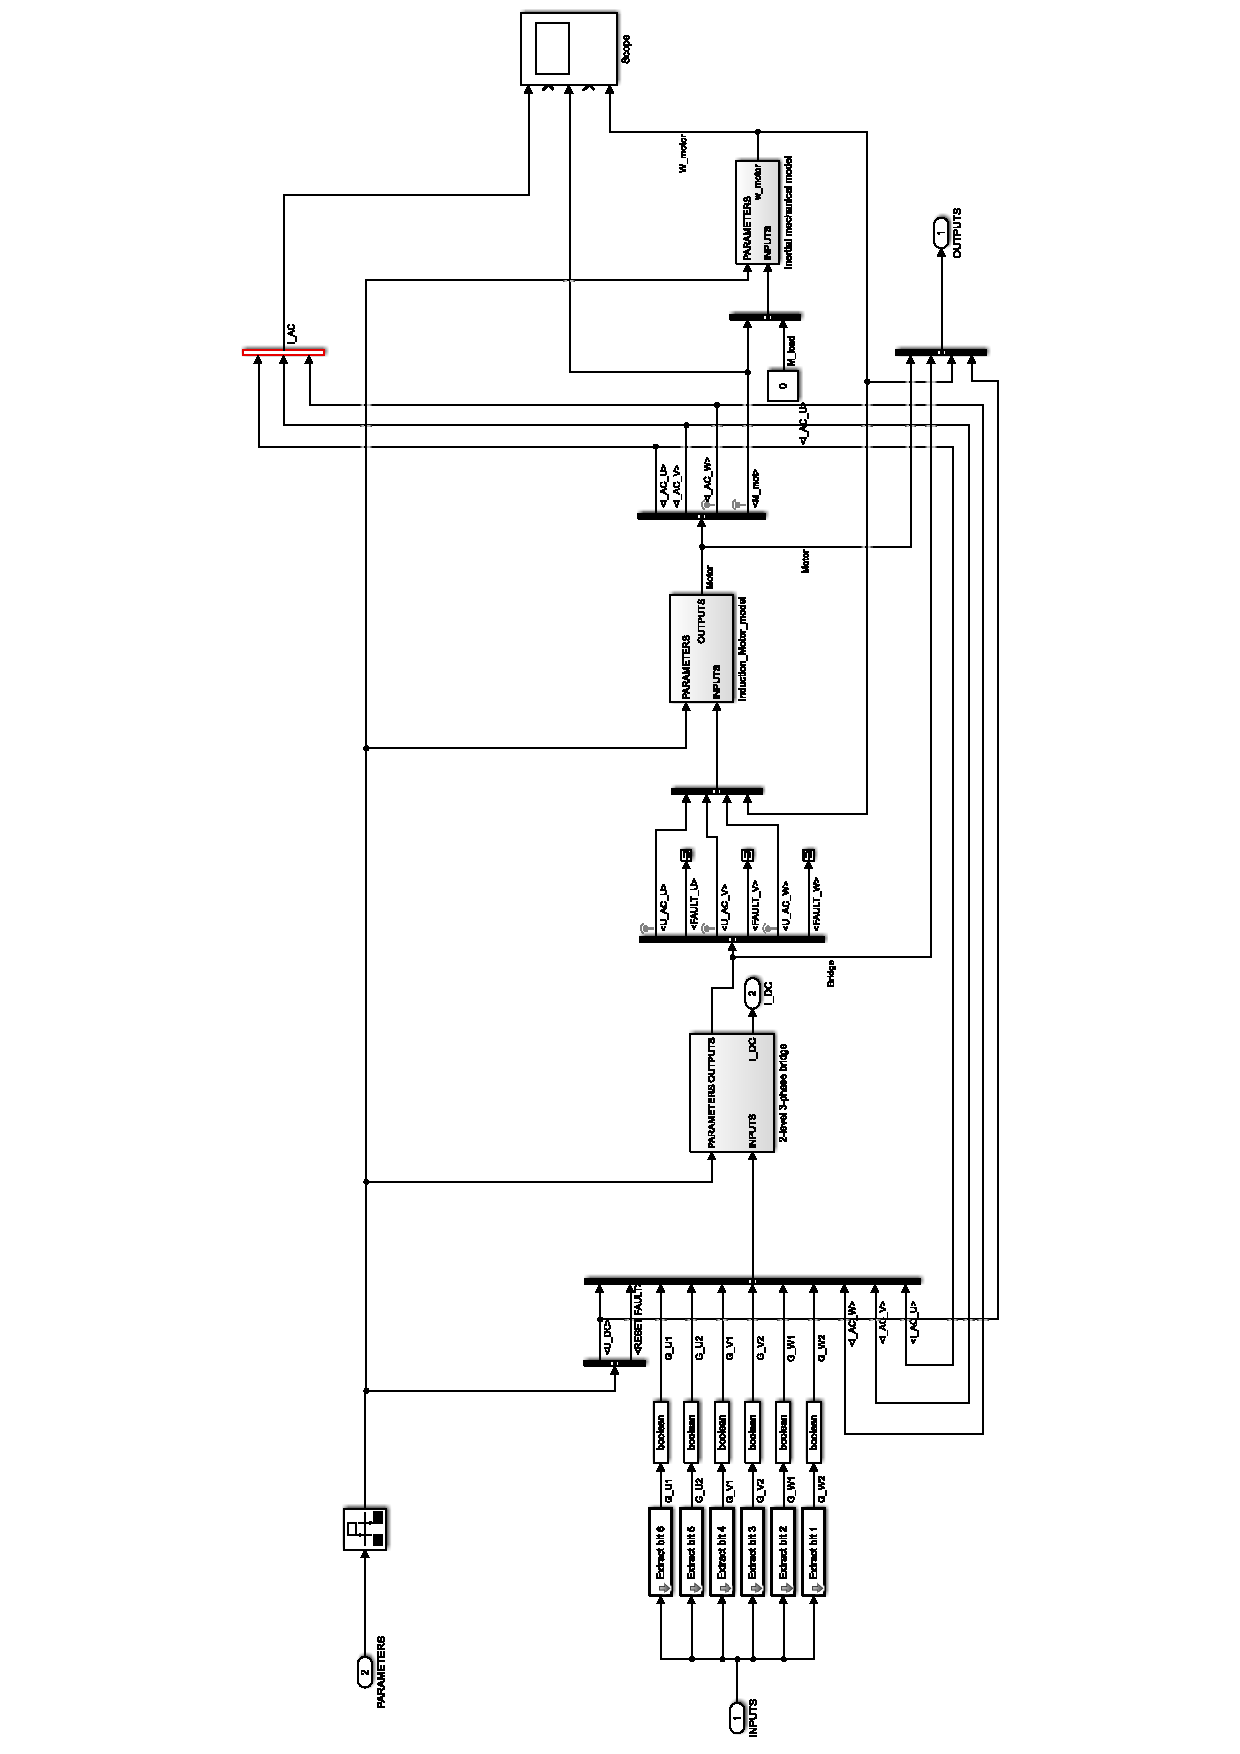
\includegraphics[width = \textwidth]{figures/hil_model.pdf}
	\caption{A SIMULINK model} 
	\label{fig:original_model}
\end{figure}

Az $I_{DC}$ terhelő áramot az alábbi egyenletek segítségével határozhatjuk meg:

\begin{equation}
\centering
I_{DC}
=
\begin{cases}
I_{AC}   & ha \  PWM_H = 1 \  | \  PWM_H = 0 \  \& \  I_{AC} < 0 \\
0 & 
\end{cases}   
\end{equation}

A módosítások \aref{fig:igbt_model}. ábra alsó részén láthatóak. Ebből a modellből valóstja meg együttesen három darab az inverter kimeneti fokozatának modelljét. 

\begin{figure}[]
	\centering
	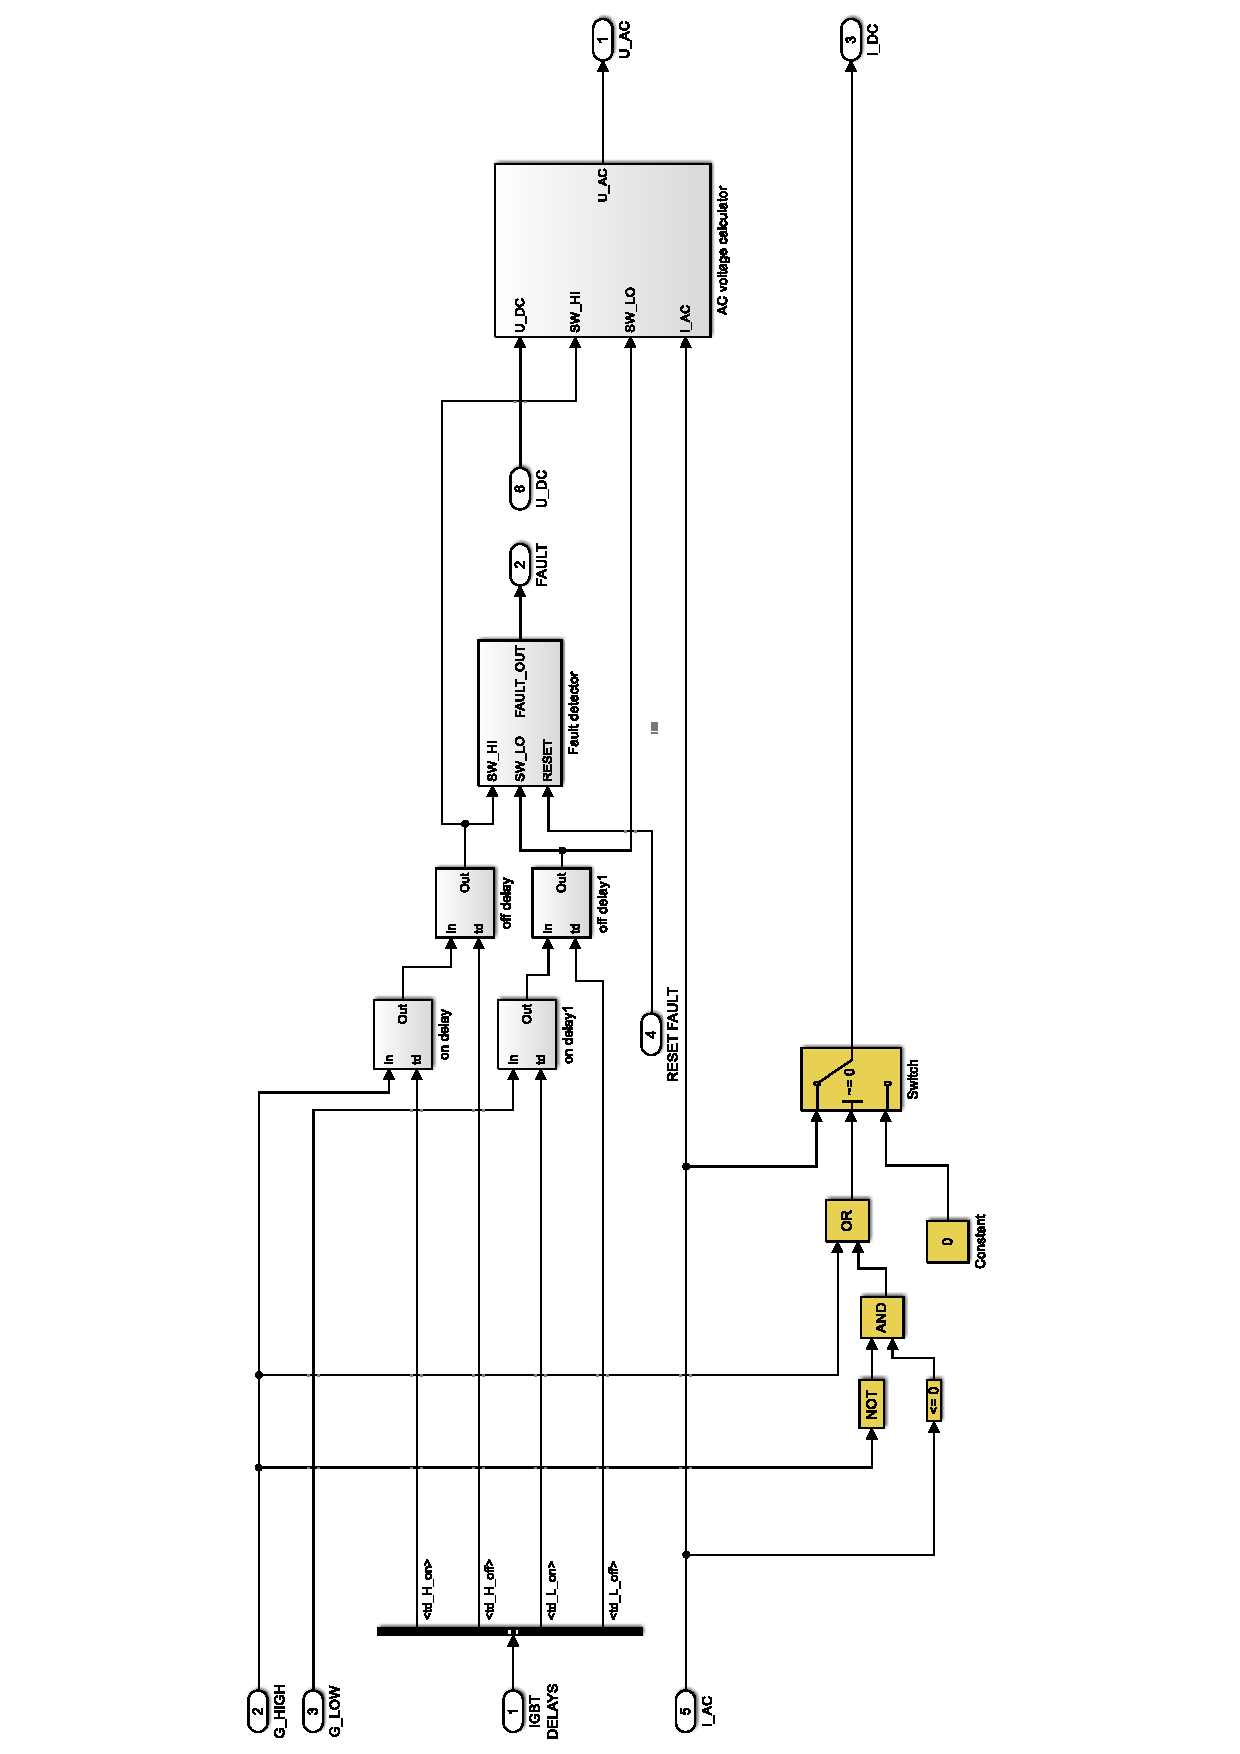
\includegraphics[width = \textwidth]{figures/igbt_model.pdf}
	\caption{A módosított félhíd modell} 
	\label{fig:igbt_model}
\end{figure}




\subsection{Az implementált bemeneti modell}

\begin{figure}[]
	\centering
	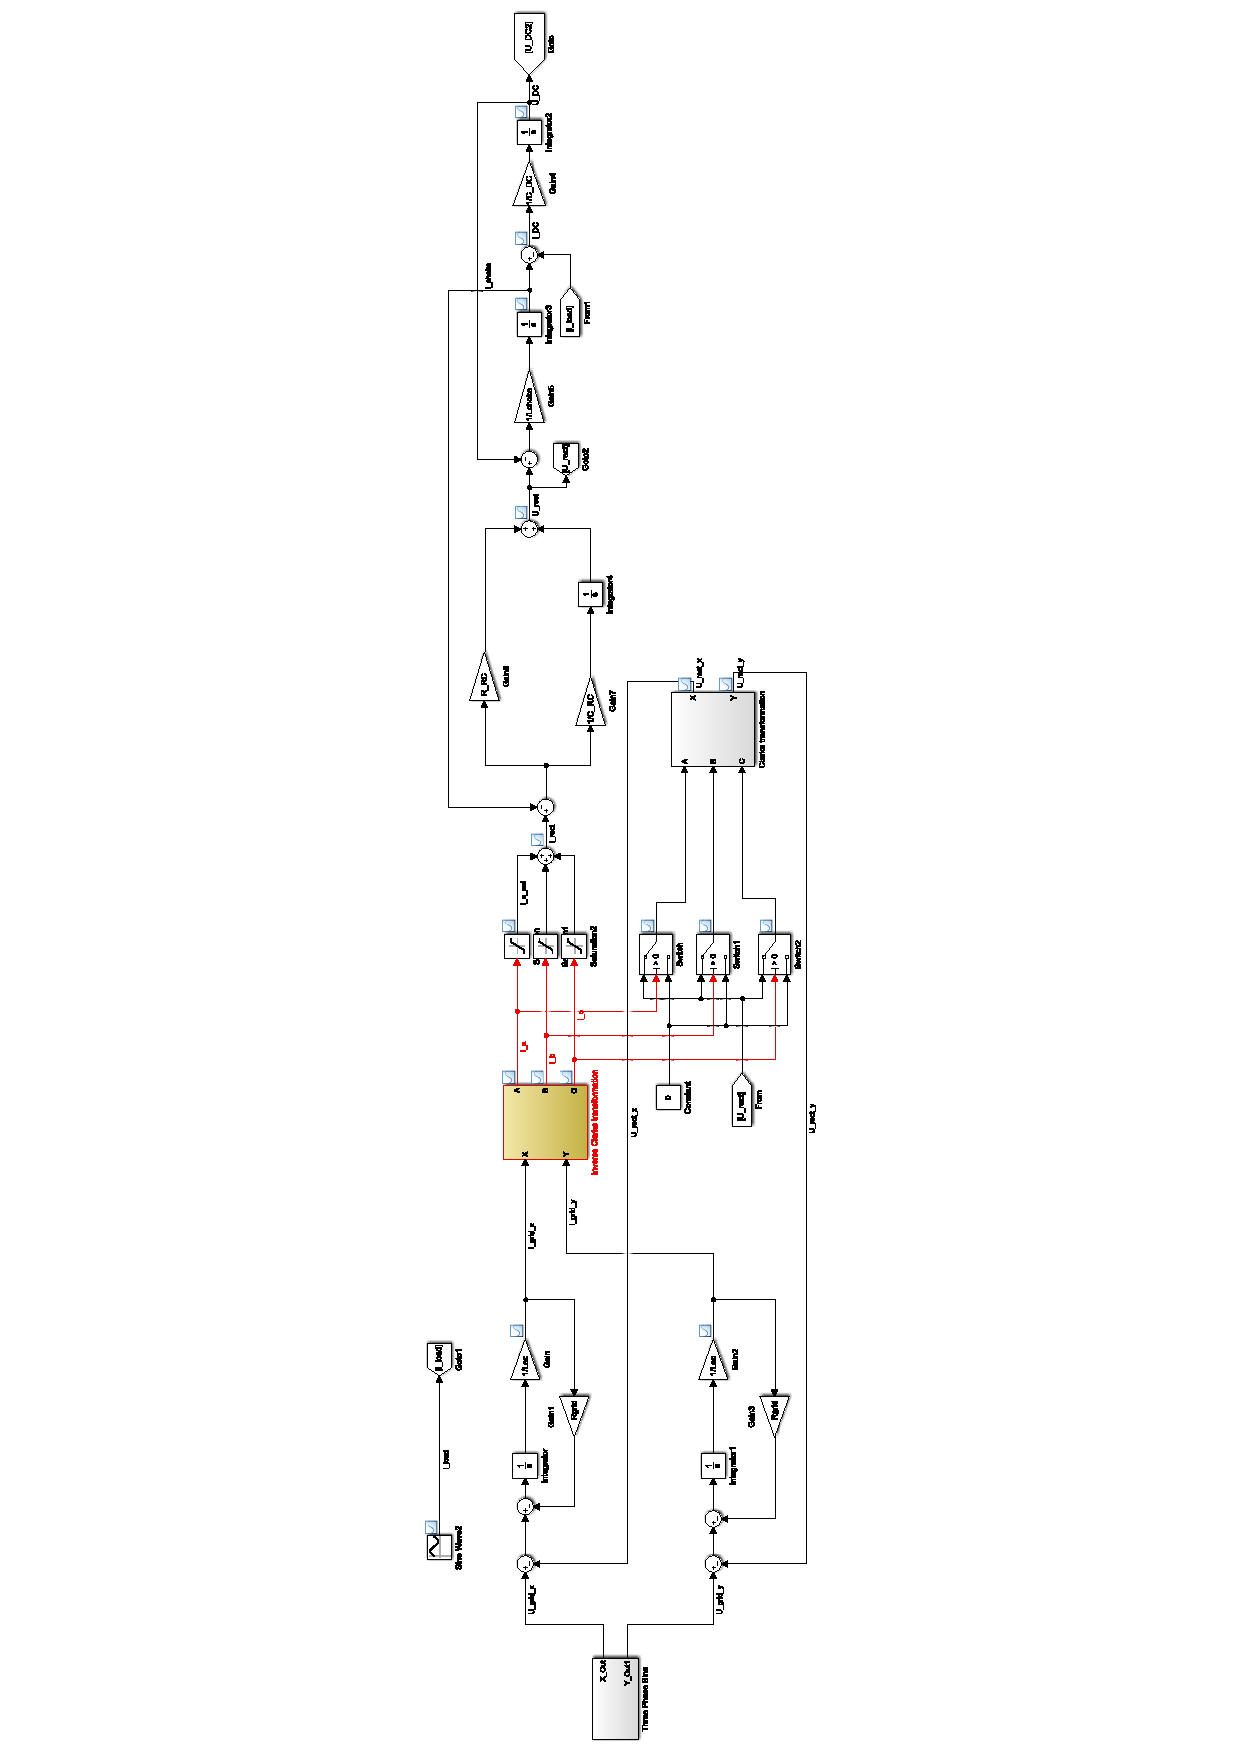
\includegraphics[width = 1.2\textwidth]{figures/model_continous.pdf}
	\caption{A frekvenciaváltó bemenetének folytonos modellje} 
	\label{fig:cont_input_model}
\end{figure}

A feladat tehát az, hogy a korábbi modellt egészítsem ki egy olyan blokkal ami a felsorolt hiányosságokat orvosolja. Az elkészítendő modellnek tartalmaznia kell tehát egy három fázisú hálózat modellt, a diódás hidat, a bemeneti DC fojtót, illetve a DC link kondenzátort. A modellezendő főáramkőri részt \aref{fig:input_marked} ábrán jelöltem. 

\begin{figure}[H!]
	\centering
	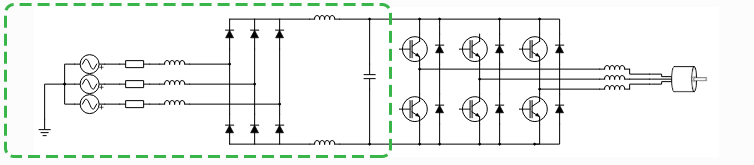
\includegraphics[width = \textwidth]{figures/VFDschematic_choke_marked.png}
	\caption{A frekvenciaváltó bemenetének folytonos modellje} 
	\label{fig:input_marked}
\end{figure}

Az első lépés a hálózat modellezése. Ehhez szükségünk van egy szinuszos feszültség előállítására. Mivel a hálózatot egy soros RL modell adja, melynek átviteli függvénye az alábbi.

\todo[inline]{Ez így nagyon nem jó}

\begin{equation}
I(s) = \frac{U(s)}{R+Ls}
\end{equation}

Mivel a három fázis induktivitása nem független egymástól, ezért az egyes fázisok egymásra hatását is figyelembe kell venni a szimuláció során. Ez jelentős számításbeli többletet jelenteni, a modell struktúráját is bonyolítaná, ezért a fázisokat inkább szétcsatoljuk és az $x,y$ koordináta-rendszerben ábrázoljuk őket. Emiatt a szinusz generátor modulban már egyből egy szinuszt és koszinuszt hozunk létre, azaz két szinusz hullámot, $90°$ fáziskülönbséggel. Ezt a két jelet vezetjük át egy-egy R-L blokkon megkapva így a hálózati áramokat. Azért, hogy visszakapjuk a három fázisú mennyiségeket, inverz Clarke transzformációt alkalmazunk a két jelent, így előáll a három fázis árama, mely a diódás híd bemenetéül szolgál.

\begin{equation}
\centering
\begin{bmatrix}
       U_a\\[0.3em]
       U_b\\[0.3em]
       U_c          
\end{bmatrix}
=
\begin{bmatrix}
       1 & 0 & 1  \\[0.3em]
       -\frac{1}{2} & \frac{\sqrt{3}}{2} & 1  \\[0.3em]
       -\frac{1}{2} & -\frac{\sqrt{3}}{2} & 1 
\end{bmatrix}
\begin{bmatrix}
       U_x\\[0.3em]
       U_y\\[0.3em]
       U_0,,        
\end{bmatrix}    
\end{equation}

\begin{equation}
\centering
\begin{bmatrix}
       U_x\\[0.3em]
       U_y\\[0.3em]
       U_0 
\end{bmatrix}
=
\begin{bmatrix}
       \frac{2}{3} & -\frac{1}{3} & -\frac{1}{3}  \\[0.3em]
       0 & \frac{1}{\sqrt{3}} & -\frac{1}{\sqrt{3}}  \\[0.3em]
       \frac{1}{3} & \frac{1}{3} & \frac{1}{3}    
\end{bmatrix}
\begin{bmatrix}
       U_a\\[0.3em]
       U_b\\[0.3em]
       U_c    
\end{bmatrix}
\end{equation}

A Clarke transzformáció arra szolgál, hogy egyszerűsítsük a három fázisú rendszerekben elvégzendő számításokat, mivel a három jellemző mennyiséget csupán kettővel reprezentálja. További előnye, hogy a nulla sorrendű komponensek a számítások során kiesnek, amire jelen esetben csak akkor lenne szükségünk, ha föld zárlatot is kívánnánk szimulálni.

A diódás modell nagyon leegyszerűsített, csak azon üzem állapotát reprezentálja a 3 fázisú 2 utas, 6 ütemű egyenirányítónak, amikor két dióda vezet benne. Ezt pedig úgy valósítjuk meg, hogy mind a három fázis negatív tartományát levágjuk, ezek után pedig az áramok összegezhetővé válnak, így előállítva az $I_{rect}$ egyenirányított áramot. A diódákon eső feszültséget pedig úgy állítjuk elő, hogy ahhoz a diódához, amelyik éppen vezet, hozzárendeljük az $U_rect$ egyenirányított feszültséget. A hálózatra való visszahatás kiszámításához azonban az így kapott három fázisú mennyiséget vissza kell alakítanunk $x,y$ tartomány-beli mennyiségekké, erre szolgál a Clark transzformáció.

Ezen a ponton két problémába is ütközünk: a diódás hídnak nincs olyan állapota, hogy egyik dióda sem vezet, emiatt a DC kondenzátorunk a végetlenségig töltődik. A jövőben tervezem a modell további finomítását, ehhez egy állapot gépet kell majd megvalósítani, a modell demonstrációs jellegére való tekintettel azonban most mást megoldást választottam. Empirikus úton kiderül, hogy a kondenzátort minimum $350\ mA$-el terhelni kell, hogy ne integrálódjon el, hanem stabilizálódjon az értéke.

A másik probléma abból adódik, hogy DC fojtó modelljének feszültség bemenetre van szüksége, és áram kimenetet ad, a diódás hídnak pedig áram kimenete van. Más struktúrájú modellel lehetséges így is megvalósítani a szimulációt, azonban egyszerűbb szétválasztani ezeket az állapot változókat egy virtuális RC-tag bevezetésével. Ennek segítségével az egyenirányító és a fojtó között is megjelenik a modellben egy potenciál. Az RC-tag paramétereit úgy választjuk meg, hogy az a modell valós működését ne befolyásolja. Úgy is tekinthetünk erre a tagra, mint egy PI szabályzóra, mely az induktivitáson eső feszültséget igyekszik $0$-ra szabályozni, felvéve a DC-link kondenzátor feszültségét.

\begin{equation}
\frac{1}{RC} \ll f_{sim}
\end{equation}

\begin{equation}
\frac{1}{\sqrt{LC}} = R
\end{equation}

\todo[inline]{Ez nem így van, csak placeholder}

\begin{figure}[H!]
	\centering
	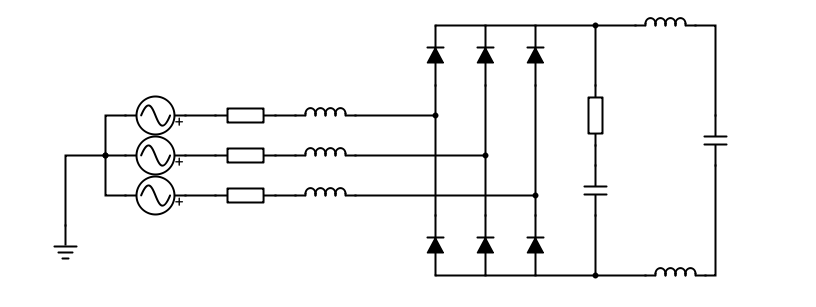
\includegraphics[width = \textwidth]{figures/VFD_virtual_RC.png}
	\caption{A frekvenciaváltó modellezett szakasza} 
	\label{fig:virtualRC}
\end{figure}

Az így kiszámolt áramból kivonva a terhelés áramát meg kapjuk a DC kondenzátort töltő áramot.

A fent leírtak alapján kialakult modell paraméterei \aref{tab:parameters}. táblázatban láthatóak. A DC fojtó induktivitását úgy kell érteni, hogy a valós rendszerben a negatív és a pozitív sínen is van egy-egy fojtó, azonban a modellben ez a kettő egyesítésre került.

\begin{table}[H]
\centering
\begin{tabular}{lS}
Hálózati feszültség            & $325\ V$ 		\\
Hálózati ellenállás            & $2\ m\Omega$   \\
Hálózati induktivitás          & $20\ \mu{}H$    			\\
DC fojtó induktivitása         & $2 \cdot{} 3\ mH$    			\\
DC link kondenzátor kapacitása & $270\ \mu{}F $   
\end{tabular}
\caption{A modell paraméterei}
\label{parameters}
\end{table}

\begin{figure}[H]
	\centering
	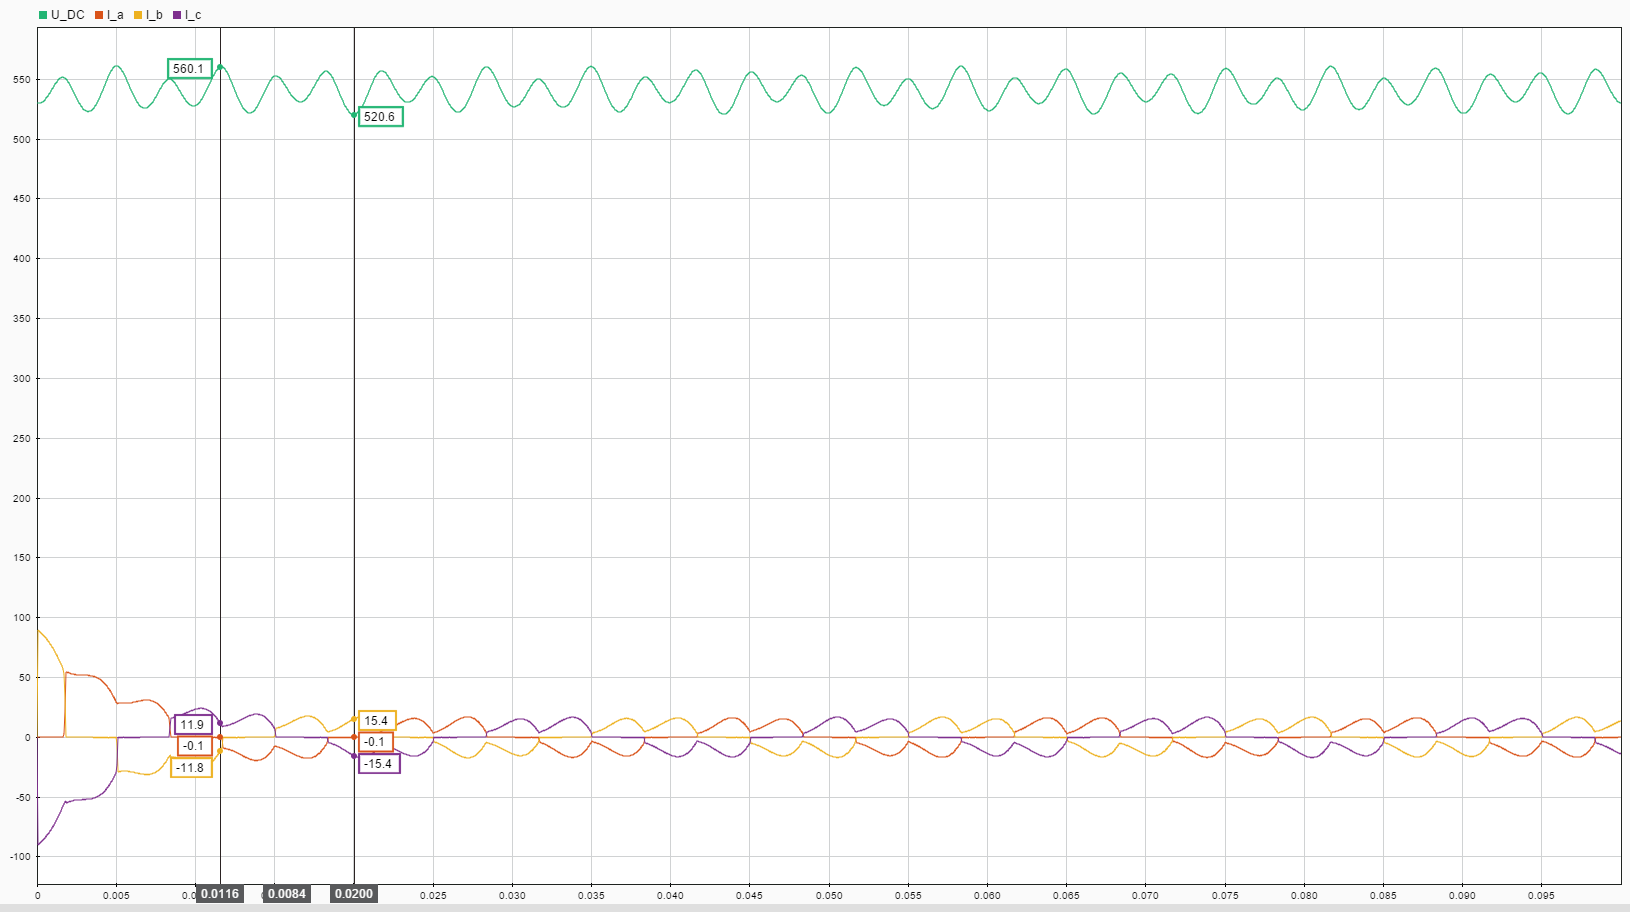
\includegraphics[width = \textwidth]{figures/continous_testrun_1.png}
	\caption{A modell által szimulált eredmények} 
	\label{fig:cont_run}
\end{figure}

\subsection{A DC fojtó szerepe}

A frekvenciaváltók bemeneti fokozatára vagy DC vagy AC oldalon szokásos fojtót alkalmazni. Enélkül a DC kondenzátor, mint kis impedanciás terhelés jelenne meg a hálózat felé. Ha felteszünk egy ipari környezetben szokásos $1,6\ MVA$-s hálózatot, egyértelművé válik, hogy a hálózatból nagyságrendekkel nagyobb áramot ki tudunk venni, mint a frekvenciaváltó üzemi értékei, ebből adódóan a kondenzátor minden kommutációnál óriási áram tüskékkel töltődne. Az induktivitás ezeket a tüskéket simítja el, csökkentve a DC kondenzátort érő áram hullámosságot és a feszültség hullámosságot is. \Aref{fig:chokenochoke}. ábrán látható egy DC fojtóval ellátott és egy anélküli szimuláció eredménye. Látható, hogy a fojtóval ellátott esetben jelentősen kisebb a DC hullámosság, valamint az áram jelalakja is sokkal simább.

\begin{figure}[H!]
	\centering
	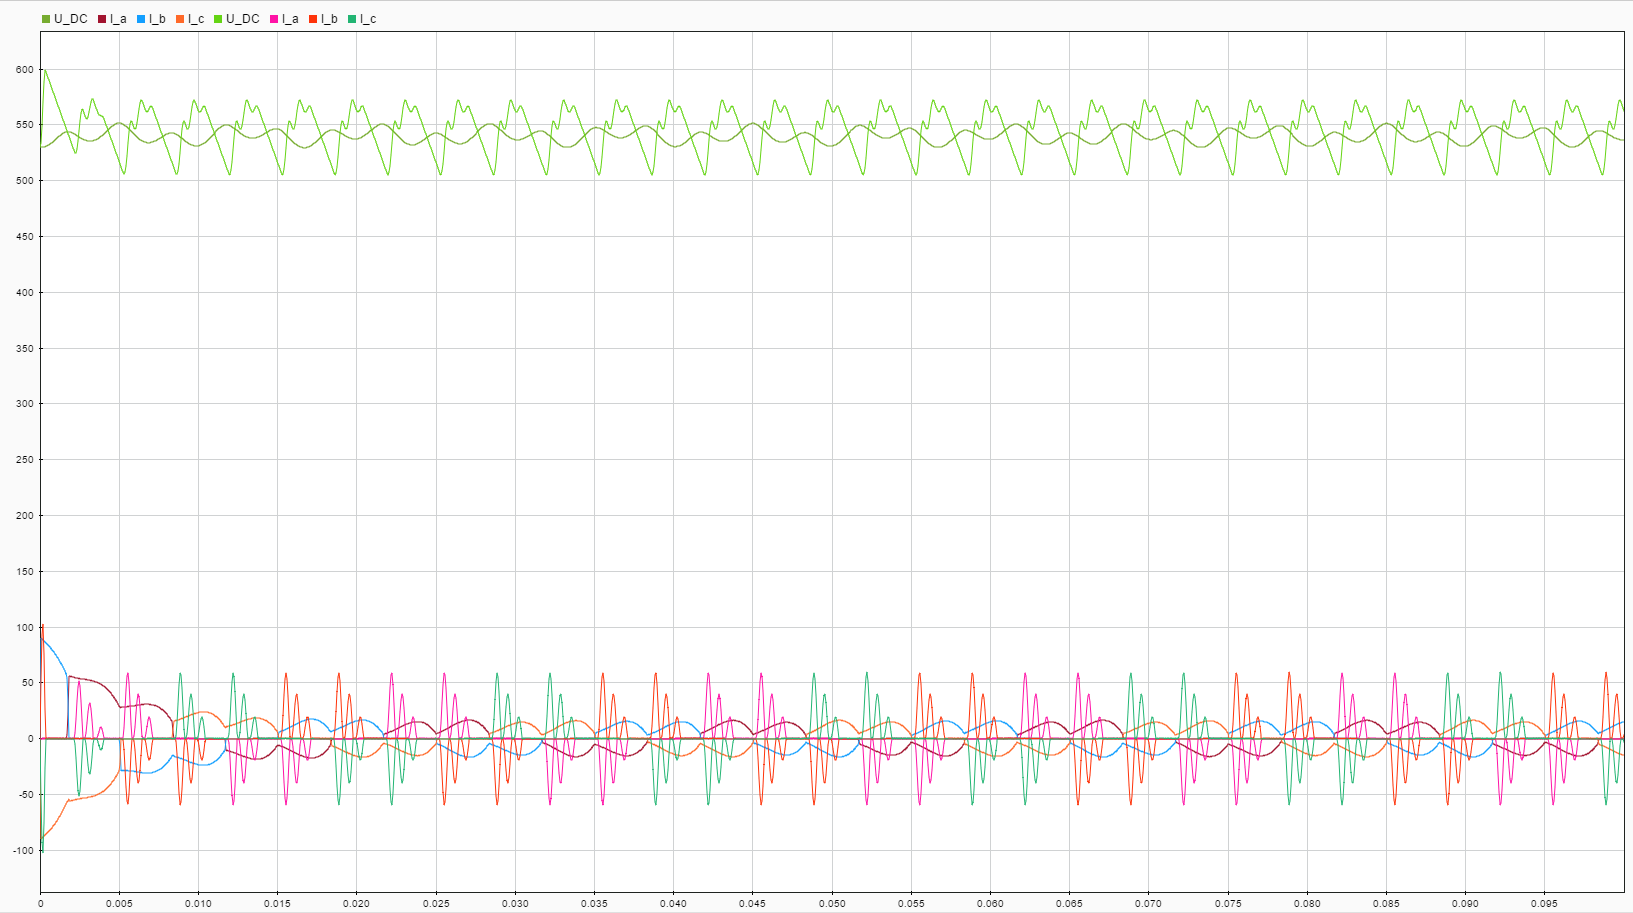
\includegraphics[width = \textwidth]{figures/choke_vs_nochoke_11A.png}
	\caption{A DC fojtó szerepe} 
	\label{fig:chokenochoke}
\end{figure}



\subsection{Áttérés diszrét időre}

Az eddig megvalósított hálózat modell folytonos idejű, Laplace tartományban ábrázolt egyenletekkel. Az FPGA, mint minden digitális rendszer azonban diszkrét időben fogja ezeket megoldani. Emiatt a modellt át kell transzformálni \emph{z} tartományba. Az integrátor matematikailag az alábbi alaknak felel meg:

\begin{equation}
\centering
\frac{1}{s} \Rightarrow \frac{1}{1-z^{-1}}
\end{equation}

Ez az átalakítás a modellben grafikusan pedig az alábbi módon jelentkezik:

\begin{figure}[h]
	\centering
	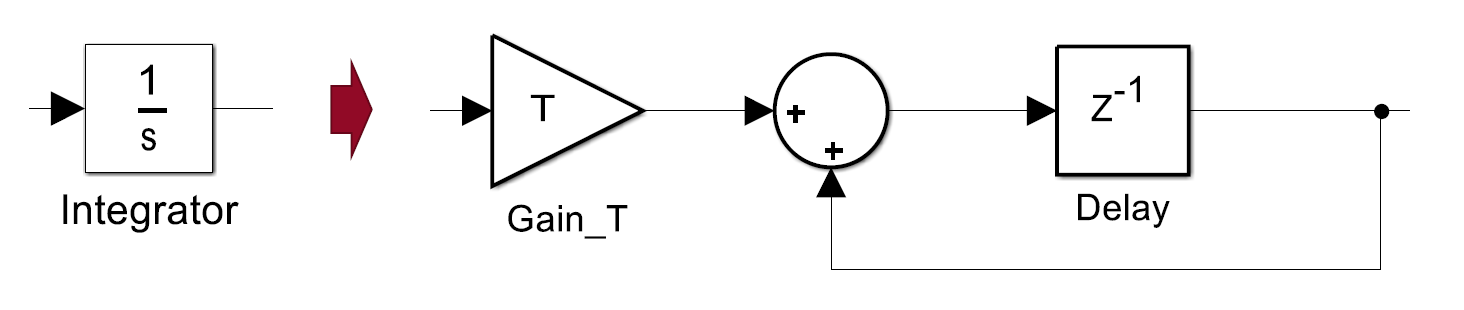
\includegraphics[width = \textwidth]{figures/integrator.png}
	\caption{Az integrázor diszkrét idejű megvalósítása} 
	\label{fig:integrator}
\end{figure}

Tehát az összes integrátor blokkon el kell végezni a fenti átalakítást.

\todo[inline]{Itt még ki kéne egészíteni z tartomány beli rizsával}

\subsection{Fixpontos ábárzolás}

Az FPGA-ban hatékonyan csak fixpontos aritmetika valósítható meg, így a most lebegőpontos változóinkat át kell alakítanunk fixpontosra. Ez könnyen megoldható, hiszen az egyes változók értéktartománya előre ismert, például tudjuk, hogy a DC feszültség biztosan kisebb, mint $U_{DC}=1000\ V$.

A lebegőpontos számábrázolás megkülönböztet egyszeres (floating) és kétszeres (double) precizitást. Előbbi a számot 32 utóbbi pedig 64 biten tárolja.

\begin{figure}[H]
	\centering
	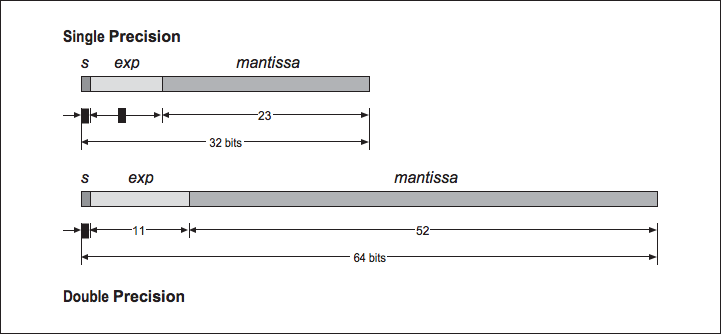
\includegraphics[width = 0.8\textwidth]{figures/floating.png}
	\caption{A lebegőpontos számábrázolás} 
	\label{fig:floating}
\end{figure}

Ilyen módon a floating körülbelül 7, a double pedig 17 tizedes jegy pontosságot enged meg. Mindkét ábrázolás mód 1 darab előjel bitet használ, ami után mantissza és exponens formájában tárolja a szám abszolút értékét. A mantissza normál alakban, a kettedes pont mögötti biteket tárolja. A normál alak biztosítja, hogy a kettedes pont előtt már csak garantáltan 1 darab 1-es van, így ez információ veszteség nélkül elhagyható. Az exponens pedig a kettedes pont helyét tárolja úgy, hogy a valós kitevő 127-el csökkentve van.

A fixpontos ábrázolás ezzel szemben rögzíti a tizedespont helyét, valamint azt nem kódolja a változóban, hanem a típusa határozza meg az értelmezés módját. A MATLAB-nak saját fixpontos formátuma van, melyet a \emph{fixdt(s,b,f)} formátummal használhatunk. Az \emph{s} jelöli, hogy az adott szám előjeles-e vagy sem, ha 1 az értéke akkor igen, ha 0, akkor nem. A következő \emph{b} a bitek számát jelöli összesen, tehát itt adhatjuk meg, hogy hány biten legyen ábrázolva a szám. Ha az adott szám előjeles, akkor nem adódik hozzá a mérethez még egy bit az előjel miatt, hanem 1 bittel csökken a szám tárolására felhasználható hely. Az utolsó \emph{f} szám jeleni a kettedes jegyek számát. Néhány példa \aref{tab:fixdt}. táblázatban látható.

\begin{table}[]
\centering
\begin{tabular}{|l|l|l|}
\hline
MATLAB típus  & tartomány               & LSB \\ \hline
fixdt(0,32,0) & 0..4294967296           & 1   \\ \hline
fixdt(1,32,0) & -2147483648..2147483648	& 1   \\ \hline
fixdt(0,8,10) & 0..0,25        	   	    & 0,0009765625 \\ \hline
fixdt(0,8,8)  & 0..1     			 	& 0,00390625    \\ \hline
fixdt(1,8,2)  & -31..32     			& 0,25    \\ \hline
\end{tabular}
\caption{A MATLAB fixpontos formátumai}
\label{tab:fixdt}
\end{table}

A Simulink alap beállításként double változóként hozza létre a jeleket és dolgozik velük. Az FPGA-val való kompatibilitás miatt azonban át kell térni fixpontos ábrázolásra. Ennek a feladatnak a megkönnyítésére a MATLAB tartalmazza a \emph{Fixpoint Advisor} nevű eszközt, azonban ilyen kis méretű modell esetében az eszköz jó felparaméterezése tovább tarthat, mint maga a megvalósítás. Az egyes változók határai látszanak a vizsgált érték tartományból. Ezen felül korlátot jelent még maga a hardver, mivel az FPGA maximum egy 18 és egy 25 bites számot tud összeszorozni. A minimális bit szám miatt tehát a pontosság és az ábrázolható érték tartomány között kell megtalálni az egyensúlyt.

\begin{table}[]
\centering
\begin{tabular}{|l|l|l|}
\hline
Jel  					&		 tartomány              & választott adattípus \\ \hline
Hálózati feszültség (V) & -1000-1000          	 		& fixdt()\\ \hline
Hálózati áram (A) 		& -50..50						& fixdt()\\ \hline
DC áram 				& -50..50        	   	   		& fixdt() \\ \hline
DC feszültség  			& 0..1000     			 		& fixdt(0,18,6)    \\ \hline
\end{tabular}
\caption{A vizsgált jeltartományok}
\label{tab:values}
\end{table} 

\todo[inline]{Ezt még ki kell számolgatni}

A kezdeti értékek meghatározása után azonban a modellen belüli számítások elvégezéséhez is meg kell találnunk a megfelelő típusokat. Ennek érdekében célszerű megvizsgálni, hogy az egyes műveletek milyen változást okoznak az ábrázolandó tartományban.

Összeadás esetén ha $fixdt(1,n,f1)$ és $fixdt(1,n,f2)$ típusú számokat adunk össze $(f1 < f2)$, esetén el kell dönteni, hogy a pontosság csökkenhet-e. Amennyiben igen, használhatjuk a továbbiakban a kevesebb törtrész bitet használó típust. Ha nem engedhető meg az ábrázolás pontosságának csökkenése $fixdt(1,n+f1-f2,f1)$ típust kell választani kimenetként. Bár a tároláshoz szükséges bitek száma megnő, nem történik sem túlcsordulás és nem vesztünk az ábrázolási pontosságból sem.

Szorzás esetén az eredményhez szükséges bitek számának változását az operandus kettes alapú logaritmusával számíthatjuk. A tört rész bitek száma $-log_2\abs{a} = m$ bittel nő a törtrész bitek száma. A kimeneti változó típus tehát $fixdt(s,n,f+m)$.

Integrálás esetén ütközünk jelentősebb problémába (és a Fixpoint Advisor is itt vérzik el), mivel ebben az esetben nagyon kis számokat kell akkumulálni. A folytonos összegzés miatt az eredmény nagyra nőhet, a pontosságot azonban úgy kell megválasztani, hogy ábrázolható legyen az inkrement. Szerencsére összeadni több biten is lehet az FPGA-ban, így nem okoz problémát nagyobb típust választani, azonban az integrátor után vissza kell konvertálni 18 biten ábrázolható méretre, még ha ezzel a pontosságból veszítünk is.

\subsection{HDL kódgeneráció}

Miután sikeresen diszkretizáltuk a modellt és a megfelelő szám ábrázolást is beállítottuk az összes változóra, készen állunk a verilog fájlok előállítására. Ehhez szükséges a Matlab HDL Coder toolboxa. Amennyiben rendelkezünk ezzel, a HDL Workflow Advisor lesz a segítségünkre a folyamat elvégzésében.

\begin{figure}[h!]
	\centering
	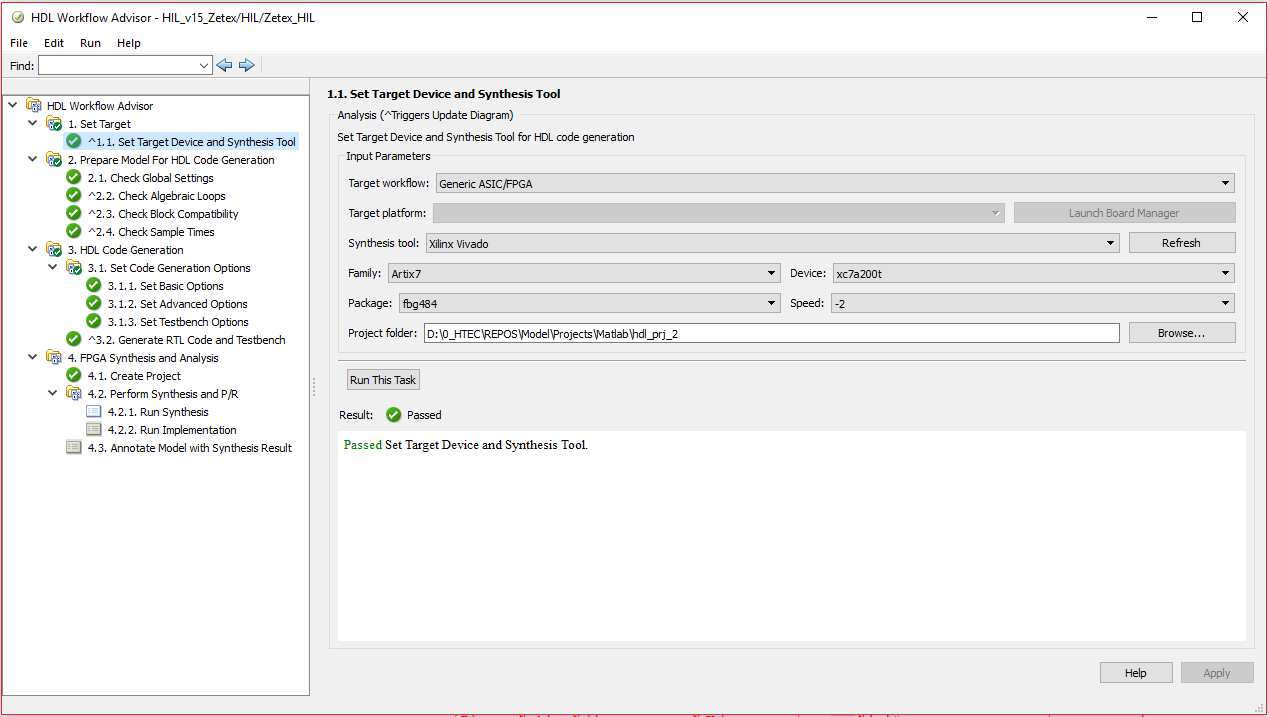
\includegraphics[width = 0.8\textwidth]{figures/hdl_advisor.png}
	\caption{A HDL workflow advisor ablaka} 
	\label{fig:hdl_advisor}
\end{figure}

Első lépésben be kell állítani, hogy milyen típusú FPGA-ra szeretnénk kódot generálni, valamint be kell állítani, hogy hova készüljön el a projekt. Ezek után a szoftver még egyszer ellenőrzi, hogy a modellből lehet-e HDL kódot generálni. Ellenőrzi, hogy van-e esetleg nem támogatott blokk a modellben, van-e algebrai hurok, illetve az időzítések megfelelőek-e. Ha minden teszt sikeres volt, akkor egyben le is futtathatjuk a taskokat a projekt létrehozásáig, a többi lépésre nincsen szükség. Ezzel előáll a verilog projekt, és ha minden sikeres volt az alábbi ablak fogad minket.

\begin{figure}[h!]
	\centering
	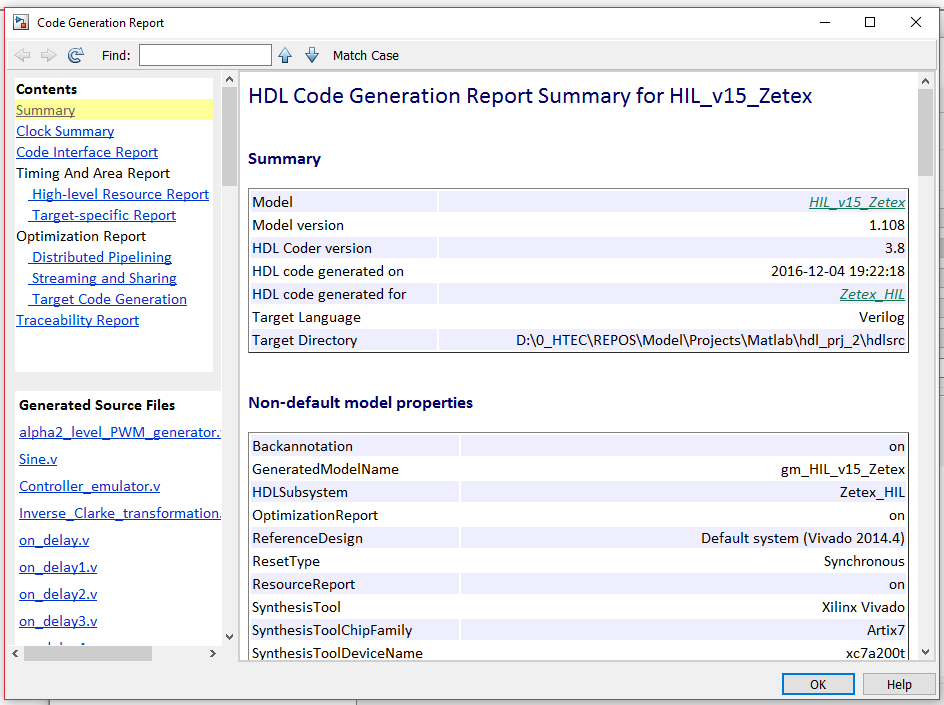
\includegraphics[width = 0.8\textwidth]{figures/hdl_report.png}
	\caption{A folyamat végi üzenet} 
	\label{fig:hdl_report}
\end{figure}

Itt megnézhetjük újra, hogy milyen beállításokkal készült el a projekt, illetve megtekinthetjük a kimeneti fájlokat is. A generált kód jól strukturált, bár kevéssé olvasható. Az egyes blokkok egy-egy modulként fordulnak le, melyeket a fő modul példányosít.

A következő lépésben Vivadoban létre kell hozni a keret rendszert adó kódot, majd ebbe integrálva a most készült modellt, generálhatjuk és az FPGA-ba töltendő bitstream-et.

\subsection{Vivado projekt}

A vivado projektben a következő feladataink vannak a modellel kapcsoaltban:
\begin{enumerate}
	\item{Példányosítani kell a ZTEX\_HIL blokkot}
	\item{Monitorozási lehetőséget kell biztosítani}
	\item{Az FPGA I/O portjait megfelelően be kell állítani}
\end{enumerate}

A példányosítás a top\_module.v fájlban történik. Megfelelő projekt beállításokkal, ha mindig ugyan oda generáljuk az új modellt, ehhez a részhez a továbbiakban csak akkor kell hozzányúlni, ha a ki vagy bemenetek módosulnak.

\begin{figure}[H]
	\centering
	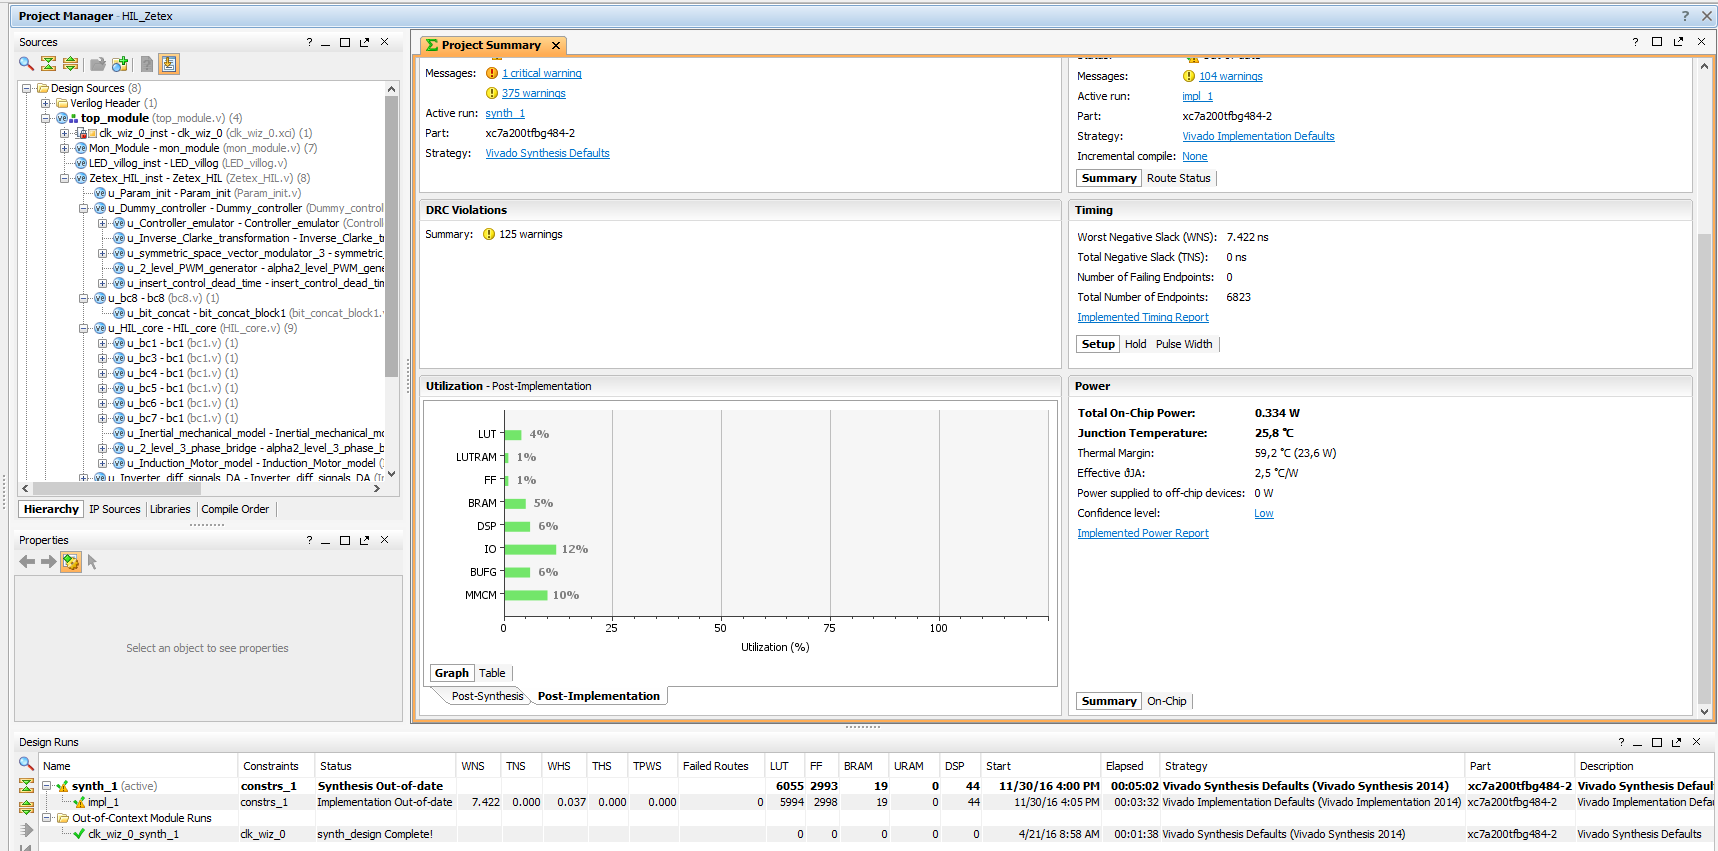
\includegraphics[width = 0.8\textwidth]{figures/vivado.png}
	\caption{A Vivado környezet} 
	\label{fig:hdl_report}
\end{figure}

A monitorozást a már több helyen bevált HiTERM program segítségével valósítottam meg. A szoftver beágyazott folyamatok megfigyelésére biztosít lehetőséget. Soros porton kommunikál az eszközzel, a megfelelő memória címekről olvas periodikusan változókat, illetve megfelelő konfiguráció esetén módosítani is lehet azokat.